\documentclass[12pt]{article}

\usepackage{graphicx}
\usepackage{float}
\usepackage{booktabs}
\usepackage{hyperref}
\usepackage{xcolor}
\usepackage{listings}
\usepackage{geometry}
\usepackage{amsmath}
\usepackage{amsthm}

\geometry{margin=1in}

% Code style
\definecolor{backcolour}{rgb}{0.95,0.95,0.95}
\definecolor{codegreen}{rgb}{0,0.6,0}
\definecolor{codegray}{rgb}{0.5,0.5,0.5}
\definecolor{codepurple}{rgb}{0.58,0,0.82}

\lstdefinestyle{mystyle}{
	backgroundcolor=\color{backcolour},
	commentstyle=\color{codegreen},
	keywordstyle=\color{magenta},
	numberstyle=\tiny\color{codegray},
	stringstyle=\color{codepurple},
	basicstyle=\footnotesize,
	breaklines=true,
	numbers=left,
	numbersep=5pt,
	showspaces=false,
	showstringspaces=false,
	showtabs=false,
	tabsize=2
}
\lstset{style=mystyle}

\title{\textbf{Analysis of Drug Overdose Deaths in the United States}}
\author{Applied Statistics II}
\date{\today}

\begin{document}
	
	\maketitle
	\thispagestyle{empty}
	
	\begin{abstract}
		This report analyzes provisional counts of drug overdose deaths in the United States using national-level mortality data from the National Vital Statistics System found on Healthcare.gov.The report focuses on four major drugs fentanyl, heroin, cocaine, and methamphetamine to evaluate total mortality, yearly trends, and recent reductions in overdose deaths. Results indicate that fentanyl is the dominant contributor to overdose mortality and is the primary driver of recent changes in overall overdose deaths.
	\end{abstract}
	
	\newpage
	
	\tableofcontents
	\newpage
	
	% ------------------------------------------------
	\section{Executive Summary}
	
	Drug overdoses remain one of the leading causes of injury-related deaths in the United States. This analysis examines national trends in overdose mortality across four major drugs: fentanyl, heroin, cocaine, and methamphetamine.
	
	Key findings include:
	
	\begin{itemize}
		\item Fentanyl accounts for the largest total number of overdose deaths across the dataset period.
		\item Over time, fentanyl's annual death count increased substantially and represents a growing share of total overdose mortality.
		\item The recent decline in overdose deaths between 2024 and 2025 is primarily driven by reductions in fentanyl-related deaths.
	\end{itemize}
	
	These results demonstrate that fentanyl dominates the overdose epidemic and largely determines overall mortality trends.
	
	% ------------------------------------------------
	\section{Data Overview}
	
	The dataset was obtained from healthdata.gov and contains provisional 12-month ending counts of drug overdose deaths based on data from the National Vital Statistics System.
	
	The following data preparation steps were implemented:
	
	\lstinputlisting[language=R, firstline=1, lastline=13]{Data Project.R}
	
	\begin{itemize}
		\item Filtered to jurisdiction labeled ``United States'' to analyze national trends.
		\item Selected only observations labeled ``12 month-ending'' to ensure consistency.
		\item Removed observations with missing overdose death values.
		\item Restricted analysis to four major drugs: fentanyl, heroin, cocaine, and methamphetamine.
		\item Converted the month-ending date variable into proper date format for yearly aggregation.
	\end{itemize}
	

	\section{Results}
	
	% ------------------------
	\subsection{Figure 1: Total Overdose Deaths by Drug (All Years)}
	
		The first figure displays the total cumulative overdose deaths for each drug across the entire dataset period.
	
	\lstinputlisting[language=R, firstline=15, lastline=28]{Data Project.R}
	
	\begin{figure}[H]
		\centering
		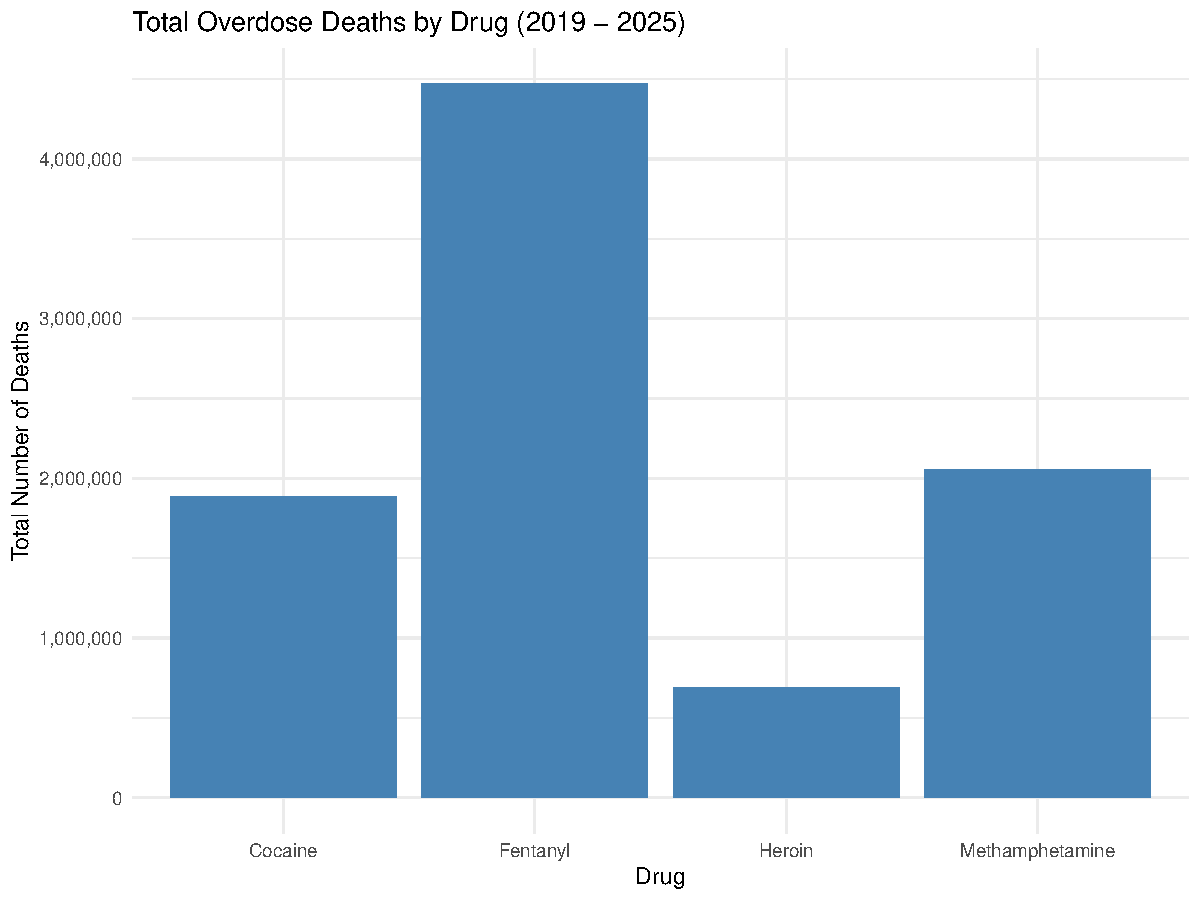
\includegraphics[width=0.8\textwidth]{plot1.pdf}
		\caption{Total Overdose Deaths by Drug Across All Years}
	\end{figure}
	
	Fentanyl accounts for the largest cumulative number of overdose deaths, far exceeding heroin, cocaine, and methamphetamine.
	
	% ------------------------
	\subsection{Figure 2: Yearly Overdose Deaths by Drug}
	
	The second figure presents annual overdose deaths for each drug using a lollipop-style visualization. Percent labels indicate fentanyl’s share of total deaths each year.
	
		\lstinputlisting[language=R, firstline=30, lastline=63]{Data Project.R}
	
	\begin{figure}[H]
		\centering
		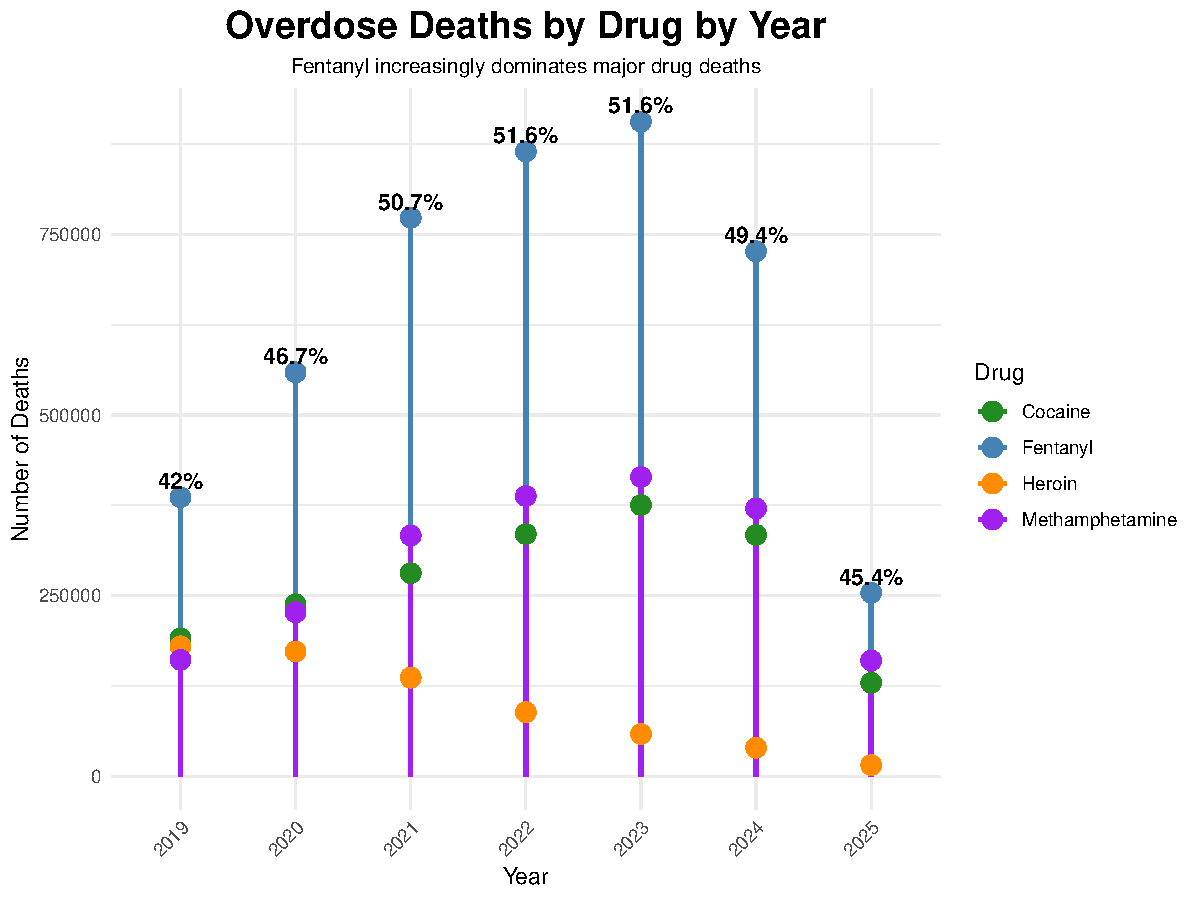
\includegraphics[width=0.9\textwidth]{plot2.pdf}
		\caption{Annual Overdose Deaths by Drug}
	\end{figure}
	
	The figure demonstrates that fentanyl deaths increased substantially over time and account for an increasing share of annual overdose mortality.
	
	% ------------------------
	\subsection{Figure 3: Reduction in Deaths from 2024 to 2025}
	
	The final figure compares total overdose deaths in 2024 and 2025 for each drug. This figure investigates the reason behind the decrease in overdoses from 2024-2025.
	
	\lstinputlisting[language=R, firstline=66, lastline=118]{Data Project.R}
	
	\begin{figure}[H]
		\centering
		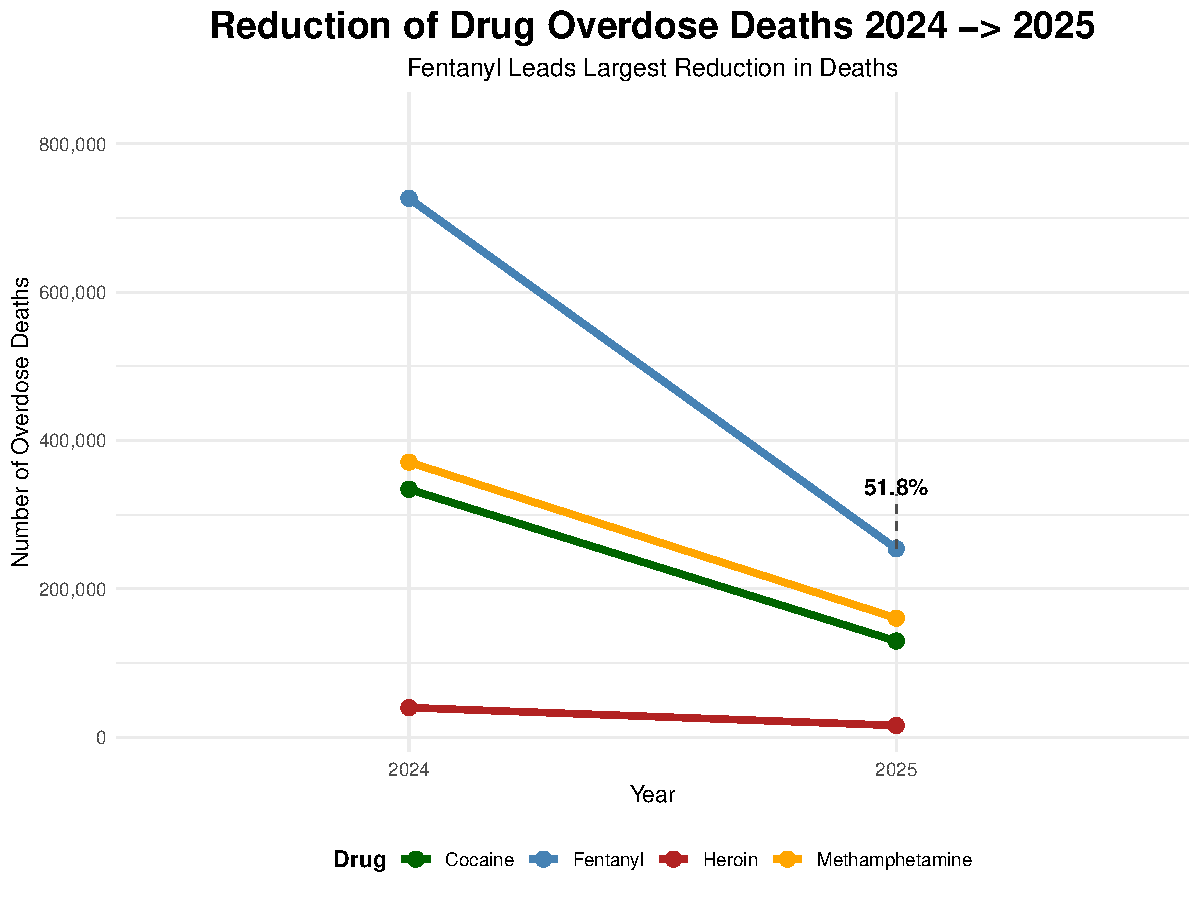
\includegraphics[width=0.9\textwidth]{plot3.pdf}
		\caption{Reduction in Drug Overdose Deaths from 2024 to 2025}
	\end{figure}
	
	The slope graph shows that fentanyl contributes the largest share of the total reduction in overdose deaths between 2024 and 2025.
	
	% ------------------------------------------------
	\section{Conclusion}
	
	This analysis demonstrates that fentanyl is the dominant contributor to overdose mortality in the United States. It accounts for the highest total number of deaths and drives both increases and decreases in overall overdose trends.
	
	While other drugs contribute to mortality, changes in fentanyl-related deaths have the greatest impact on national overdose totals. Policies and interventions targeting fentanyl may therefore yield the most substantial reductions in overall overdose mortality.
	
\end{document}